\PassOptionsToPackage{svgnames}{xcolor}

\documentclass[11pt,a4paper]{article}


% português BR
\usepackage[brazilian]{babel}
\usepackage[utf8]{inputenc}
\usepackage[T1]{fontenc}

% Para o flow chart
\usepackage{tikz}
\usetikzlibrary{shapes.geometric, arrows}
\usepackage{dcolumn}


\usepackage{adjustbox}

\usepackage{threeparttable}

% box
\usepackage{float} 
\usepackage{tcolorbox}
\tcbuselibrary{skins,breakable}

\newenvironment{myblock}[1]{%
    \tcolorbox[
    % beamer,%
    noparskip,
   % breakable,
    colback=LightCoral,
    colframe=DarkRed,%
   % colbacklower=Tomato!75!LightCoral,%
    title=#1]}%
    {\endtcolorbox}

% formas no flow chart
\tikzstyle{startstop} = [rectangle, rounded corners, minimum width=3cm, minimum height=0.5cm,text centered, draw=black, fill=red!30]
\tikzstyle{process} = [rectangle, minimum width=3cm, minimum height=0.5cm, text centered, draw=black, fill=orange!30]
\tikzstyle{io} = [trapezium, trapezium left angle=70, trapezium right angle=110, minimum width=2cm, minimum height=0.5cm, text centered, draw=black, fill=blue!30]
\tikzstyle{arrow} = [thick,->,>=stealth]


\title{Importância das distribuidoras para o sucesso de público dos filmes de ficção nacionais entre 2001 e 2013}

% para a tabela das variáveis booleanas
\usepackage{multirow}


\begin{document}

\maketitle


\section{Objetivo}

Discriminar e quantificar o impacto das distribuidoras sobre o público nos filmes ficcionais brasileiros no mercado doméstico.


\section{Material e Métodos}

Os métodos utilizados no estudo estão resumidos na Figura \ref{fig:fluxograma}. Descrições detalhadas de cada etapa estão apresentadas abaixo.
 

\begin{figure}
\centering
% flow chart
\begin{tikzpicture}[node distance=1.5cm]

\node (start) [startstop] {Começo};
\node (coleta) [process, below of=start] {Coleta de dados realacionados aos filmes};
\node (filtro) [process, below of=coleta] {Remoção de filmes de acordos com filtros};
\node (normal) [process, below of=filtro] {Normalização e transformação dos dados};
\node (label) [process, below of=normal] {Separação dos dados em grupos};

\node (grupo2) [io, below of=label, xshift=-4cm] {Grupo Booleano};
\node (grupo1) [io, below of=label] {Grupo Numérico};
\node (grupo3) [io, below of=label, xshift=4cm] {Grupo Distribuidoras};

\node (modelo1Construcao) [process, below of=grupo1] {Construção de um modelo de regressão linear múltipla};
\node (modelo1) [io, below of=modelo1Construcao] {Modelo 1};
\node (modelo2Construcao) [process, below of=modelo1] {Adição das variáveis do Grupo Booleano ao modelo via regressão logística};
\node (modelo2) [io, below of=modelo2Construcao] {Modelo 2};

\node (modelo3Construcao) [process, minimum width=12cm, below of=modelo2] {Adição das variáveis do Grupo Distribuidoras ao modelo via regressão logística};

\node (modelo3) [io, below of=modelo3Construcao] {Modelo 3};
\node (impacto) [process, below of=modelo3] {O coeficiente cada distribuidora no modelo é interpretado como impacto desta no público};
\node (fim) [startstop, below of=impacto] {Fim};

\draw [arrow] (start) -- (coleta);
\draw [arrow] (coleta) -- (filtro);
\draw [arrow] (filtro) -- (normal);
\draw [arrow] (normal) -- (label);

\draw [arrow] (label) -- (grupo1);
\draw [arrow] (label.west) -| (grupo2);
\draw [arrow] (label.east) -| (grupo3);

\draw [arrow] (grupo1) -- (modelo1Construcao);
\draw [arrow] (modelo1Construcao) -- (modelo1);
\draw [arrow] (modelo1) -- (modelo2Construcao);
\draw [arrow] (grupo2.west) -| (modelo2Construcao.west);
\draw [arrow] (modelo2Construcao) -- (modelo2);
\draw [arrow] (modelo2) -- (modelo3Construcao);
\draw [arrow] (modelo3Construcao) -- (modelo3);
\draw [arrow] (grupo3.east) -| (modelo3Construcao.east);
\draw [arrow] (modelo3) -- (impacto);
\draw [arrow] (impacto) -- (fim);

\end{tikzpicture}
\caption{Fluxograma resumido dos método utilizado no estudo}
\label{fig:fluxograma}
\end{figure}


\subsection{Coleta de dados relacionados aos filmes}

Dados referentes aos filmes lançados no periodo de 2001 à 2013 foram obtidos em bancos de dados de organizações governamentais (ANCINE; Ministério da Justiça), sites relacionados à cinema (IMDB, Rotten Tomatoes, adorocinema, etc) e em periódicos (Veja, Folha de São Paulo, Estadão, etc). A tabela presente no arquivo \textit{tabela1A.csv} (anexado) contém todos os dados levantados e as respectivas fontes das informações.


\subsection{Remoção de filmes de acordo com filtros}

Filmes foram removidos se:

\begin{enumerate}

 \item Eram documentários.
 \item Não possuiam informação de variáveis usadas no modelo.
 \item Eram relançamentos.

O número de filmes removidos e as causas estão na Tabela \ref{table:motivoRemocao}. Dos 1020 filmes 598 foram removidos.


\end{enumerate}

\begin{table}
\centering
\begin{tabular}{{l}{r}}

Motivo da remoção & Quantidade de filmes \\
\hline
Eram Documentários & 373 \\
Ausência do valor captado junto a ANCINE & 141\\
Ausência de avaliação qualitativa do filme & 1\\
Ausência do público do filme & 2\\
Eram relançamento & 81\\
\hline

\end{tabular}

\caption{Quantidade de filmes removidos do estudo de acordo com as causas.}
\label{table:motivoRemocao}

\end{table}

\subsection{Normalização e transformação dos dados}


Os valores captados junto à ANCINE foram ajustado segundo a inflação para valores de dezembro de 2013 utilizando os índices fornecidos pelo Instituto de Pesquisa Econômica Aplicada (IPEA).

As notas qualitativas dos filmes segundo periódicos ou \textit{site} foram normalizadas e arrendondas para o número intergral mais próximo no intervalo de 1 à 3. Isso porque as fontes destas notas são múltiplas, com diferentes intervalos de pontuações e, pressumidamente, possuem heterogenidade nos critérios de avaliação. 

Campos multivalorados foram transformados em variáveis booleanas de acordo com a presença ou ausência da variável nos filmes (ver caixa \textit{Campos multivalorados à campos booleanos}). Para evitar aumentar o número de comparações e também para incrementar a robustez dos testes somente se analissou variáveis booleanas contidas em mais de 8 filmes. A lista das variáveis booleanas após o filtro e o número de filmes em que elas estão presentes se encontram na Tabela \ref{table:booleanas}.

\vspace*{0.2cm}


\begin{myblock}{Campos multivalorados à campos booleanos}
Para exemplificar processo vamos usar o campo \textit{atores} dos filmes \textit{Tropa de Elite 2} e \textit{O Caminho das Nuvens}. Os Atores principais de cada filme estão listados abaixo:

\vspace*{0.2cm}

\textbf{\textit{Tropa de Elite 2}}
\begin{itemize}
\item Wagner Moura
\item Maria Ribeiro
\end{itemize}

\textbf{\textit{O Caminho das Nuvens}}
\begin{itemize}
\item Cláudia Abreu
\item Wagner Moura
\item Ravi Ramos Lacerda
\end{itemize}

A presença ou não de cada ator (Wagner Moura, Maria Ribeiro, Cláudia Abreu e Ravi Ramos Lacerda) será representada em um campo. Nesse o valor \textit{1} será atribuído aos filmes que apresentam o ator e o valor \textit{0} aos filmes que não o apresentam. 

Dessa forma ao invés da notação:

\vspace*{0.5cm}

\resizebox{\textwidth}{!}{%
\begin{tabular}{{l}{r}}
Filme & Atores \\
\hline
Tropa de Elite 2 &  W. Moura / M. Ribeiro \\
O Caminho das Nuvens & C. Abreu / W. Moura / R. Lacerda\\
\hline
\end{tabular}}

\vspace*{0.5cm}

Teremos a notação:

\vspace*{0.5cm}

\resizebox{\textwidth}{!}{%
\begin{tabular}{{l}{l}{l}{l}{r}}
Filme &  W. Moura & M. Ribeiro & C. Abreu & R. Lacerda\\
\hline
Tropa de Elite 2     & 1 & 1 & 0 & 0\\
O Caminho das Nuvens & 1 & 0 & 1 & 1\\
\hline
\end{tabular}}

\vspace*{0.5cm}


Essa transformação foi feita em todos os campos multivalorados (\textit{Diretores}; \textit{Atores}; \textit{Gêneros}; \textit{Distribuidoras}). As colunas com soma menor que oito foram removidas. Ou seja, só foram considerados atores diretores, gêneros ou distribuidoras com presença em pelo menos oito filmes.


\end{myblock}

\vspace*{0.2cm}



\begin{table}
\centering
\begin{threeparttable}

\begin{tabular}{ {l}{l}{r}}
Tipo & Variável &  Quantidade de filmes\\


 
\hline
\multirow{2}{*}{Diretores} 
 & Daniel Filho & 8\\ 
 & Moacyr Goes & 9\\ 
 
 
\hline 
\multirow{13}{*}{Atores} 

 & João Miguel & 8 \\
 & Mariana Ximenes & 8 \\
 & Marco Ricca & 8 \\
 & Dira Paes & 9\\ 
 & Rodrigo Santoro & 9 \\ 
 & Fábio Assunção & 9 \\
 & Lázaro Ramos & 9 \\
 & Leonardo Medeiros & 9 \\
 & Caco Ciocler & 10\\
 & Paulo José & 10\\
 & Wagner Moura & 11\\
 & Caio Blat & 11\\
 & Selton Mello & 14\\
 
 
\hline
\multirow{8}{*}{Gêneros} 

 & Infantil & 11 \\
 & Animação & 13 \\
 & Suspense & 13 \\ 
 & Ação & 16 \\
 & Aventura & 25 \\
 & Romance & 35 \\
 & Comédia & 97 \\
 & Drama & 253 \\ 

 
 \hline
\multirow{12}{*}{Distribuidoras} 

 & Estação & 10 \\
 & Paramount & 11\\
 & Paris & 11\\
 & Providence & 18 \\
 & Imovision &  20 \\
 & RioFilme &  25 \\
 & Europa &  26 \\
 & Fox &  27 \\
 & Warner Bros. & 29 \\
 & Downtown & 29\\
 & Imagem & 33 \\
 & Columbia & 52 \\
 & \textit{DO}\tnote{*} & 131 \\

 
 
 
\hline
\end{tabular}

\begin{tablenotes}
\item[*] \textit{Distribuidoras ocasionais}: Categoria atrelada aos filmes que não foram distribuídos por nenhumas das outras distribuidoras presentes.
\end{tablenotes}
\end{threeparttable}

\caption{Variáveis booleanas consideradas no estudo}

\label{table:booleanas}


\end{table}

Uma decorrência desse filtro é que somente empresas que distribuiram mais de 8 filmes (\textit{distribuidoras atuantes} -- \textit{DA}) seriam analisadas. Porém, notou-se que todas as \textit{DA} que significativamente impactavam o público o faziam de forma positiva, como será demonstrado abaixo nos resultados. Se conjecturou que como as \textit{DA} tem grande presença no mercado é esperado que elas tenham maior facilidade de distribuir e promover seus filmes do que as demais, o que explicaria o resultado. Para mensurar o impacto do filmes não serem distribuídos por uma \textit{DA} e para avaliar estas distribuidoras considerando seus tamanhos se criou a classe de \textit{distribuidoras ocasionais} (\textit{DO}). A classe \textit{DO} foi atribuída a todos os filmes que não foram distribuídos por nenhuma das \textit{DA}.

\subsection{Separação dos dados em grupos}

Os dados referentes aos filmes foram divididos em três grupos (\textit{Grupo Numérico}; \textit{Grupo Booleano}; \textit{Grupo Distribuidoras}). Essa separação foi feita pois os dados de cada um dos grupos foi adicionado ao modelo em etapas (Figura \ref{fig:fluxograma}). Os grupos estão descritos abaixo: 

\subsubsection{Grupo Numérico}

%Formado por quatro variáveis numéricas, sendo que duas (\textit{IBOPE} e \textit{Log(Público anterior)}) são consideradas somente em casos específicos:

\begin{description}

  \item[Log(captado)] \hfill \\
  Logaritmo natural dos valores captados junto à ANCINE pelo filme ajustados segundo a inflação para valores de dezembro de 2013 utilizando os índices fornecidos pelo IPEA.
  \item[Nota] \hfill \\
  Nota qualitativa do filme segundo sites especializados em cinema ou periódicos normalizadas e arrendondas para o número intergral mais próximo no intervalo de 1 à 3.
  \item[IBOPE] \hfill \\
  Caso o filme seja baseado em um programa de TV ou tenha no título o nome de uma personalidade que apresenta um programa de TV (\textit{eg}: \textit{Casseta \& Planeta: A Taça do Mundo É Nossa}; \textit{Xuxa e os Duendes}; \textit{Eliana e os Golfinhos}) se considerou a pontuação do programa na cidade de São Paulo do Instituto Brasileiro de Opinião Pública e Estatística (IBOPE) na data publicamente disponível mais próxima ao lançamento.  
  \item[Log(Público anterior)] \hfill \\
  Caso o filme seja uma sequência (\textit{eg}: \textit{Tropa de Elite 2}, \textit{Boleiros 2}), se considerou o público do filme anterior.  
\end{description}



\subsubsection{Grupo Booleano}

Grupo formado pelas variáveis booleanas dos tipos \textit{Diretores}, \textit{Atores} e \textit{Gêneros} (Tabela \ref{table:booleanas}).

\subsubsection{Grupo Distribuidoras}

Grupo formado pelas variáveis booleanas do tipo \textit{Distribuidora} (Tabela \ref{table:booleanas}).

\subsection{Construção do modelo}

A construção de um modelo para a previsão do logaritmo natural do público dos filmes foi feito em três etapas. Na primeira etapa se criou a base do modelo com variáveis declaradas \textit{a priori} importante para a previsão. Nas demais etapas se incrementou o modelo com as variáveis booleanas. Abaixo a descrição dos modelos produzidos em cada etapa:

\begin{description}

  \item[Modelo 1] \hfill \\
  Modelo de regressão linear múltipla formado por todas variáveis do \textit{Grupo Numérico}.

    \item[Modelo 2] \hfill \\
   Se incrementou o \textit{Modelo 1} com as variáveis do \textit{Grupo Booleano} usando regressão logística \textit{stepwise forward} utilizando o Critério de Informação Bayesiano (\textit{BIC}) como filtro através da função \textit{StepAIC} do pacote \textit{MASS} em \textit{R}. Se restringiu a regressão logistica para que as variáveis do \textit{Modelo 1} não fossem retirada. 

  \item[Modelo 3] \hfill \\
  Se incrementou o \textit{modelo 2} com as variáveis do \textit{Grupo Distribuidoras} usando o mesmo método e critérios utilizados para construir o \textit{Modelo 2} (inclusive restringindo  para que variáveis já presentes no modelo não fossem retiradas).
  
    \item[Modelo 3'] \hfill \\
    Assim, como no \textit{modelo 3} se incrementou o \textit{modelo 2} com as variáveis do \textit{Grupo Distribuidoras}, porém antes desse procedimento se adicionou ao modelo a variável \textit{DO}.
 
  
\end{description}


\subsection{Importância das distribuidoras}

O coeficiente estimado de cada distribuidora no \textit{Modelo 3} foi usado como estimativa do impacto da distribuidora (ou da variável \textit{DO}) no público do filme. 



\section{Resultados}

Os resultados dos modelos estão na Tabela \ref{table:resultados} e a visualização dos impactos das distribuidoras estão apresentados das Figura \ref{figure:modelo3} e na Figura \ref{figure:modelo3_2}. Abaixo a descrição dos resultados em cada um dos modelos produzidos.

\begin{table}[!htbp] 
\centering 

\begin{adjustbox}{width=0.88\textwidth}

\label{} 
\begin{tabular}{@{\extracolsep{5pt}}lD{.}{.}{-3} D{.}{.}{-3} D{.}{.}{-3} D{.}{.}{-3} } 

 & \multicolumn{4}{c}{\textit{Variável depedente: \textit{Log(Público)}}} \\ 
\cline{2-5} 

\\[-1.8ex] & \multicolumn{1}{c}{Modelo 1} & \multicolumn{1}{c}{Modelo 2} & \multicolumn{1}{c}{Modelo 3} & \multicolumn{1}{c}{Modelo 3'}\\ 
\hline \\[-1.8ex] 

  & & & & \\

 Constante & -9.725^{***} & -7.530^{***} & -4.196^{***} & -4.046^{***} \\ 
  & (1.231) & (1.178) & (1.238) & (1.246) \\ 
  & & & & \\
  
 Log(captado) & 1.278^{***} & 1.136^{***} & 0.872^{***} & 0.947^{***} \\ 
  & (0.083) & (0.078) & (0.085) & (0.080) \\ 
  & & & & \\ 
  
 Nota & 0.717^{***} & 0.887^{***} & 0.860^{***} & 0.783^{***} \\ 
  & (0.153) & (0.145) & (0.138) & (0.139) \\ 
  & & & & \\ 
  
 IBOPE & 0.160^{***} & 0.130^{***} & 0.130^{***} & 0.116^{***} \\ 
  & (0.031) & (0.028) & (0.028) & (0.027) \\ 
  & & & & \\   
  
  Log(Público anterior)  & 0.121^{***} & 0.094^{**} & 0.090^{**} & 0.097^{**} \\ 
  & (0.047) & (0.043) & (0.041) & (0.041) \\ 
  & & & & \\ 
  
  \textbf{Gêneros} & & & & \\ 
    & & & & \\   

  \quad Drama &  & -1.010^{***} & -0.869^{***} & -0.910^{***} \\ 
  &  & (0.224) & (0.215) & (0.216) \\ 
  & & & & \\ 
  
 \quad Suspense &  & -1.361^{***} & -1.544^{***} & -1.426^{***} \\ 
  &  & (0.494) & (0.471) & (0.471) \\ 
  & & & & \\ 
  
 \quad Comédia &  & 0.602^{**} & 0.374 & 0.362 \\ 
  &  & (0.250) & (0.240) & (0.242) \\ 
  & & & & \\ 
  

  \textbf{Diretores} & & & & \\ 
    & & & & \\ 
    
 \quad Daniel Filho  &  & 1.714^{***} & 1.250^{**} & 1.482^{**} \\ 
  &  & (0.616) & (0.595) & (0.589) \\ 
  & & & & \\
  
 \quad Moacyr Goes  &  & 1.477^{**} & 1.487^{***} & 1.407^{**} \\ 
  &  & (0.581) & (0.571) & (0.554) \\ 
  & & & & \\ 
  
  \textbf{Atores} & & & & \\ 
    & & & & \\   
  
  \quad Wagner Moura &  & 1.325^{**} & 1.225^{**} & 1.239^{**} \\ 
  &  & (0.531) & (0.527) & (0.507) \\ 
  & & & & \\ 
  
  
  \textbf{Distribuidoras} & & & & \\ 
    & & & & \\ 
  
  \quad Paris &  &  & 2.077^{***} &  \\ 
  &  &  & (0.505) &  \\  
  & & & & \\ 
  
 \quad Fox &  &  & 1.761^{***} &  \\ 
  &  &  & (0.356) &  \\ 
  & & & & \\ 

  
 \quad Downtown  &  &  & 1.564^{***} &  \\ 
  &  &  & (0.332) &  \\ 
  & & & & \\
  
 \quad Columbia &  &  & 1.096^{***} &  \\ 
  &  &  & (0.284) &  \\ 
  & & & & \\
  
 \quad Paramount &  &  & 1.497^{***} &  \\ 
  &  &  & (0.523) &  \\ 
  & & & & \\
  
 \quad Imagem &  &  & 0.942^{***} &  \\ 
  &  &  & (0.307) &  \\ 
  & & & & \\ 
  
 \quad Warner Bros. &  &  & 0.899^{**} &  \\ 
  &  &  & (0.357) &  \\ 
  & & & & \\   
  
  
 \quad \textit{DO} &  &  &  & -1.211^{***} \\ 
  &  &  &  & (0.195) \\ 
  & & & & \\  
  
 \quad RioFilme &  &  &  & -1.190^{***} \\ 
  &  &  &  & (0.349) \\
  & & & & \\ 

  
 \quad Providence  &  &  &  & -1.128^{***} \\ 
  &  &  &  & (0.413) \\ 
  & & & & \\
  

  
\hline \\[-1.8ex] 


Observações & \multicolumn{1}{c}{422} & \multicolumn{1}{c}{422} & \multicolumn{1}{c}{422} & \multicolumn{1}{c}{422} \\ 

R$^{2}$ & \multicolumn{1}{c}{0.446} & \multicolumn{1}{c}{0.545} & \multicolumn{1}{c}{0.601} & \multicolumn{1}{c}{0.589} \\ 

R$^{2}$ ajustado & \multicolumn{1}{c}{0.441} & \multicolumn{1}{c}{0.534} & \multicolumn{1}{c}{0.584} & \multicolumn{1}{c}{0.576} \\ 

Erro padrão residual & \multicolumn{1}{c}{1.853 (df = 417)} & \multicolumn{1}{c}{1.692 (df = 411)} & \multicolumn{1}{c}{1.599 (df = 404)} & \multicolumn{1}{c}{1.614 (df = 408)} \\ 

F & \multicolumn{1}{c}{84.063$^{***}$ (df = 4; 417)} & \multicolumn{1}{c}{49.297$^{***}$ (df = 10; 411)} & \multicolumn{1}{c}{35.744$^{***}$ (df = 17; 404)} & \multicolumn{1}{c}{44.997$^{***}$ (df = 13; 408)} \\ 


\hline 
\hline \\[-1.8ex] 
\textit{Nota:}  & \multicolumn{4}{r}{$^{*}$p$<$0.1; $^{**}$p$<$0.05; $^{***}$p$<$0.01} \\ 


\end{tabular} 

\end{adjustbox}


\caption{Resultados das regressões lineares. Na parte de cima da tabela estão expressos os coeficientes das variáveis com o erro padrão entre parênteses.}
\label{table:resultados}


\end{table} 


\subsection{Modelo 1}
Todas as variáveis indepedentes deste modelo apresentaram correlação significativa e positiva com a variável depedente. Essa correlação está de acordo com as justificativas que nos levaram a incluir \textit{a priori} esses campos. 


\subsection{Modelo 2}
A adição das variáveis booleanas (com execessão da classe \textit{Distribuidoras}) se deu através de regressão logística \textit{stepwise forward} utilizando \textit{BIC} como filtro. A formulação de modelos utilizando regressões logísticas possuem uma tendência de superajuste, ainda que se tenha tentando balancear isto com a utilização de um critério conservador (\textit{BIC}) e fixando variáveis indepedentes ao modelo (as variáveis presentes no \textit{Modelo 1}). Contundo se salienta que o \textit{Modelo 2} não possui uma função preditiva e sim de selecionar as covariáveis presentes no \textit{Modelo 3}, que por sua vez será utilizado somente como forma de mensurar o impacto das distribuidoras e não terá função preditiva. 

Nota-se que, como apontado em publicações jornalísticas, que a variável \textit{Comédia} aparece como tendo impacto significativamente positivo, enquanto os outros dois gêneros adicionados ao modelo (\textit{Drama} e \textit{Suspense}) apresentam impacto negativo. Os dois diretores analisados (Daniel Filho e Moacyr Goes) apresentaram associação significativa e positiva com a variável depedente. Importante notar que ambos os diretores estão atrelados à diversas produções ditas globais (eg: \textit{ Trair e coçar é só começar}; \textit{Xuxa e o tesouro da cidade perdida}; \textit{Xuxa abracadabra}; \textit{Xuxinha e Guto contra os monstros do espaço}; \textit{Se Eu Fosse Você}; \textit{Se Eu Fosse Você 2}; \textit{Primo Basílio}). Somente um ator demonstrou impacto significativo (\textit{Wagner Moura}) e este foi positivo.


\subsection{Modelo 3}

Tendo seleciono as covariáveis (variáveis presentes no \textit{Modelo 2}) para o estudo das variáveis depedentes de interesse um terceiro modelo foi criado adicionado as variáveis da classe \textit{Distribuidoras} através também de regressão logística \textit{stepwise forward} utilizando \textit{BIC} como filtro. Para a construção desse modelo se considerou as 12 distribuidoras que apresentavam mais de oito filmes no período (tabela \ref{table:booleanas}, classe \textit{Distribuidoras}). Destas 12 distribuidoras 7 apresentaram um impacto significativo na variável depedente, todos positivos (Tabela \ref{table:resultados} e Figura \ref{figure:modelo3}). 

  

\begin{figure}[h!]
\centering
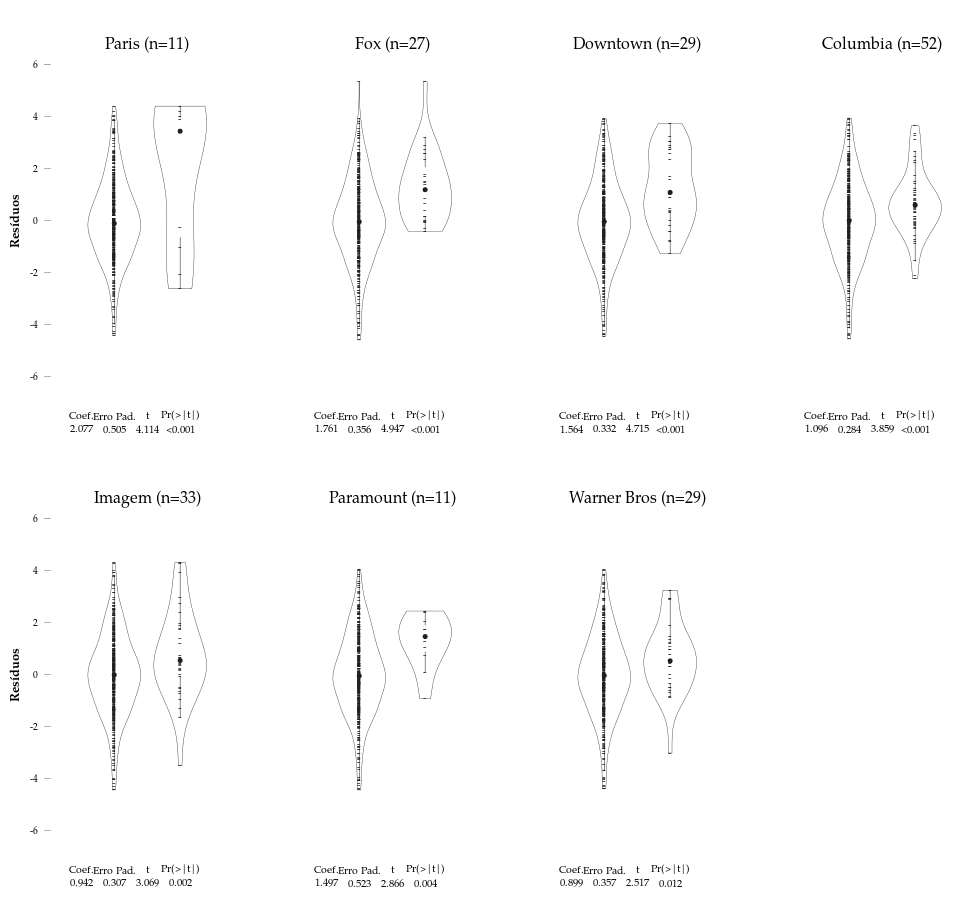
\includegraphics[width=0.9\textwidth]{figura_1.png}
 \caption{\textit{Violin plot} dos resíduos de todos os filmes e dos filmes das distribuidoras com impacto significativo no \textit{Modelo 3}. Cada gráfico representa os resíduos do \textit{Modelo 3} desconsiderando o impacto da distribuidora em questão.}
\label{figure:modelo3}
\end{figure}


\subsection{Modelo 3'}
Se conjecturou que a razão pela qual todos os impactos das variáveis da tipo \textit{Distribuidoras} serem positivos era devido ao viés de terem sido consideradas somente empresas com mais de 10 filmes no período, ou seja, distribuidoras que tem presença constante no mercado, logo com possíveis vantagens competitivas. Dentro do universo de filmes analisados essas empresas representa somente 11\% das distribuidoras, porém estão presentes em 69\% dos filmes. Como forma de inspecionar a diferença entre estas empresas e também para mensurar a importâncias delas considerando que fazem parte de um subgrupo específico se criou a classe \textit{DO} que foi atribuída à filmes distribuídos somente por empresa(s) que distribuiram menos de 10 filmes no período. 

Após contemplar o \textit{Modelo 2} com a variável \textit{DO}, sequiu-se a adição das distribuidoras através de regressão logística, tal qual no \textit{Modelo 3}. A variável \textit{DO}, como esperado, teve impacto significativo e e negativo na variável depedente. Ou seja, a distribuição por empresas não atuantes (menos de 10 filmes) apresenta relação com um menor público. Além disso dentro dos parâmetros desse modelo, duas distribuidoras (RioFilme e Providence) demonstraram um impacto negativo  significativo em relação à outras \textit{DA}.


 

\begin{figure}[h!]
\centering
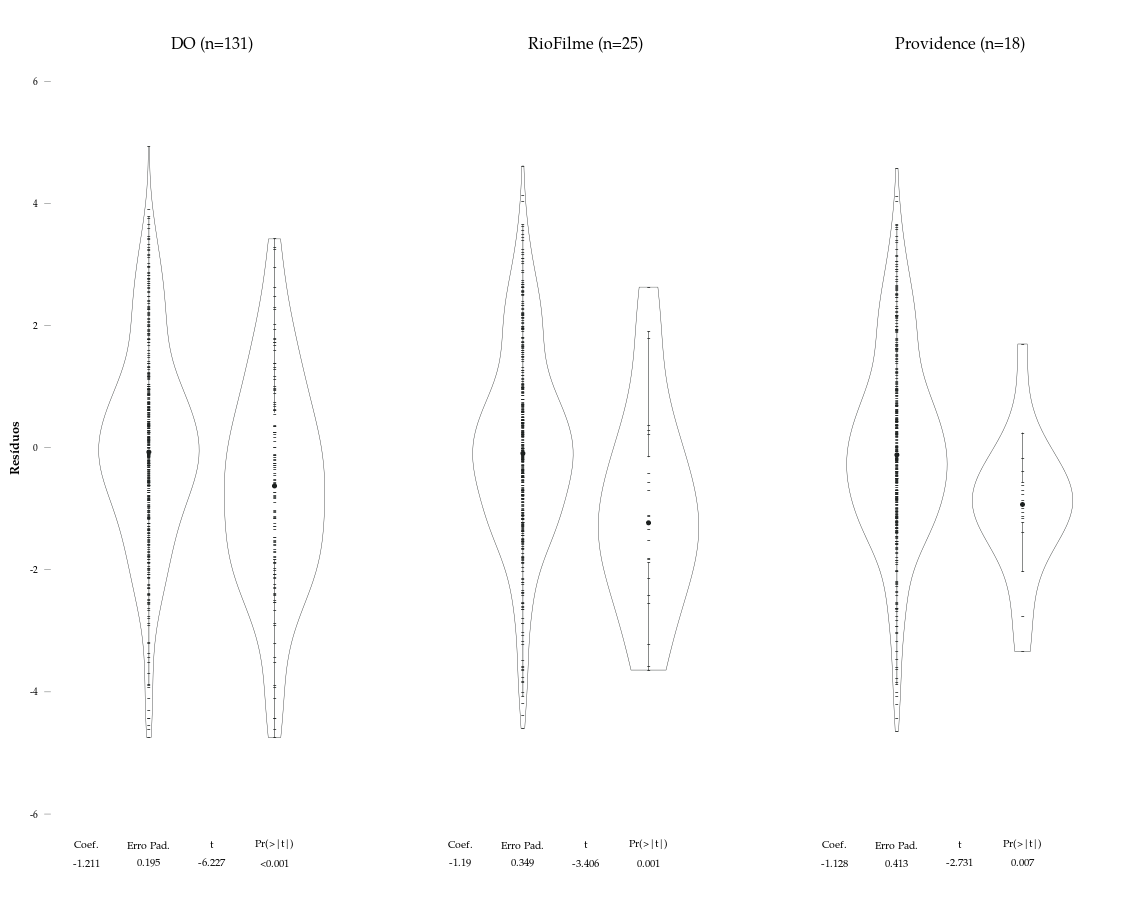
\includegraphics[width=0.9\textwidth]{figura_2.png}
 \caption{\textit{Violin plot} dos resíduos de todos os filmes e dos filmes das distribuidoras com impacto significativo no \textit{Modelo 3'}. Cada gráfico representa os resíduos do \textit{Modelo 3'} desconsiderando o impacto da distribuidora em questão.}
\label{figure:modelo3_2}
\end{figure}


\section{Conclusões}

Das 12 distribuidoras analisadas, 7 demonstraram um impacto significativo e positivo sobre o público durante o período examinado. (Tabela \ref{table:resultados} e Figura \ref{figure:modelo3}). O incremento esperado no público devido à presença das distribuidora variou de 207\% à 89\%. Uma vez estabelecido essa importância se investigou a alteração no público devido ao fato de filmes não serem distribuídos por empresas atuantes (distribuidoras com 10 ou mais filmes no período). Essa segunda análise  demonstrou que filmes que contam com pelo menos umas das duas 12 distribuidoras atuantes tendem a ter um ganho de público de 121\%. Importante ressaltar que a perda de público devido ao filme ser distribuído por uma empresa não atuante não deve ser constante entre as distintas distribuidoras que compõem o grupo, porém não foi possível mensurar o impacto individual devido ao reduzido número de filmes atrelado a cada uma das empresas no período. Outro resultao dessa segunda análise é a presença de duas distribuidoras (RioFilmes e Providence) do grupo de distribuidoras atuantes, que aparecem distoante do resto do conjunto ao impactarem significativamente menos do que as outras distribuidoras atuantes (Tabela \ref{table:resultados} e Figura \ref{figure:modelo3_2}).  

\end{document}
